\chapter{Evaluation}
This chapter contains the evaluation of our \emph{Learned Selection Strategy for Lightweight Integer Compression Algorithm Parameterizations} which is divided into three parts. Firstly, we describe our hardware setup and data sets and evaluate how long training and forward passes take. Secondly, we validate our approach against the baseline selection strategy and evaluate its performance with a validation data set. Lastly, we take a look at the feature importance in order to understand the predictions of our ML models better.
\section{Setup}
All models have been trained on a AMD Quad-Core A10-9700 APU system with 16 GB memory. The same system has been used to label the feature vectors and for application and testing of the models. The process of data labeling was necessary once by running all examples with \emph{StaticBP} and \emph{DynamicBP}. The implementation of the COLLATE metamodel by Hildebrandt et. al \cite{Hildebrandt2017} considers every different parameterization as a different algorithm and generates its implementation on the fly. This results in long compiling times before the data labeling process can start. Once labeled, the training and application of the ML model is possible.

Advantages of GB regression are the relatively fast times for training and forward passes in contrast to other methods like Neural Networks. On average, one training phase took 17.3s. Due to the fact that it was necessary to train 110 models during the hyperparameter tuning for each combination of algorithm and target value, the whole process took 127 minutes. 
For the forward passing process we measured an average duration of 390$\mu$s.

For the following validation measures, we used different data sets.
One the one hand, we used a fixed 20\% of the set generated by the La-Ola generator labeled with the compression runtime and the compression rate. This dataset is called generated data set (GDS).
On the other hand, we evaluated how our strategy performs on real-world data. Therefore we used a further data set (pBI) which consists of representative samples from the Public BI benchmark. The Public BI benchmark is a user-generated benchmark and consists of real world data represented in different tables \cite{Ghit2020}.

\section{Validation}
The ML model of our selection strategy is able to predict the optimal compression algorithm as well as the best-fitting parameters. In order to validate the quality of the predictions, we use multiple indicators. The \emph{algorithm accuracy} (aa) is the relative frequency of true positive algorithm predictions \emph{aTP} for a data set \emph{S}.   
\begin{equation} \label{eq:algo_accuracy}
    aa(aTP, S) = \frac{aTP}{|S|} \cdot 100\%
\end{equation}
Regarding the \emph{parameterization accuracy} (pa), we use the true positive predictions of the the algorithm parameters \emph{pTP}.
\begin{equation} \label{eq:param_accuracy}
    pa(pTP, S) = \frac{pTP}{|S|} \cdot 100\%
\end{equation}
Besides the calculation of the accuracy, we also consider the slowdown. It measures how much performance would be lost if the wrong prediction is chosen. As our strategy focuses on the parameterization, we decided to exclusively consider the slowdown of the wrong parameters. Having a set \emph{G} containing the target values (runtimes or compression rates) of all wrongly predicted parameterizations, a set \emph{H} containing their actual target values, and the amount of all wrongly predicted parameterizations \emph{n}, the slowdown can be calculated using the SAMPE metric.
\begin{equation} \label{eq:slowdown}
    slowdown(G,H) = \frac{200\%}{n} \sum_{i = 1}^{n} \frac{|G_{i} - H_{i}|}{|G_{i}| + |H_{i}|}
\end{equation}

In order to evaluate the quality of our ML model, a baseline is necessary. We decided to compare our model to the most simple algorithm with a parameterization allowing the compression of integer values within a range as large as possible. In particular, this baseline strategy uses \emph{StaticBP} with an input format of 64 bit and an output format of 8 bit.

The hyperparameter tuning process has shown that the hyperparameters for \emph{DynamicBP} and \emph{StaticBP} are similar. Regarding the compression rate, a more complex model is necessary for \emph{DynamicBP} in order to make predictions with the same accuracy as for \emph{StaticBP} due to the fact that the compression rate of \emph{StaticBP} can be directly derived from the parameters.

\begin{figure}[h]
    \centering
    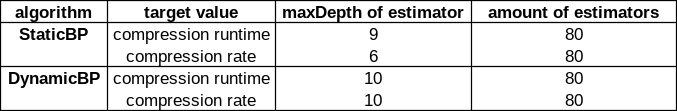
\includegraphics[scale=0.45]{hyperparameters_table}
    \caption{Result table of the hyperparameter tuning process.}
    \label{fig:table_hyperparameters}
\end{figure}

Our ML models have been trained on integer sequences with lengths of 800, 1600, 3200 and 6400 depending on the output format as described in Section \ref{ch:data_gen_pipe}. However, the input format of every integer sequence of the pBI dataset is 64 bit, but the lengths of the arrays are much bigger than the lenghts we chose for our training data. Though the sequence lengths of the pBI dataset differ for almost every sample, all of them are integer divisable by 8 what makes it possible to compress them using the COLLATE metamodel implementation by Hildebrandt et. al \cite{Hildebrandt2017}.
Due to the smaller lengths used for the training data, it is necessary to scale the predicted target value if it is proportional to the amount of integers being compressed. This is only the case for the compression runtime. The compression rate is independent of the data length. Given the output format \emph{of}, the unscaled compression runtime \emph{ur}, and the length of the integer sequence \emph{l}, we calculate the scaled runtimes (sr) for the pBI dataset according to the following equation.
\begin{equation}
    sr = \frac{ur}{of \cdot 100} \cdot {l}
\end{equation}

\begin{figure}
    \centering
    \begin{subfigure}{.5\textwidth}
      \centering
      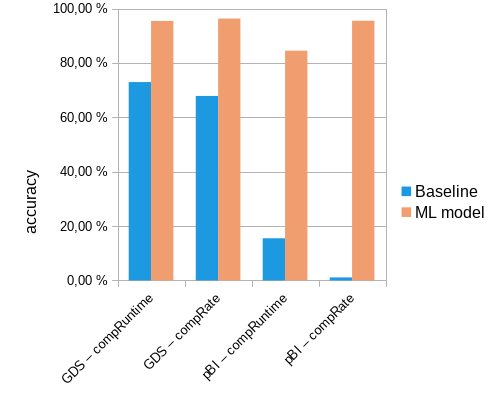
\includegraphics[scale=0.43]{accuracy_algo_new_new}
      \caption{Accuracy of algorithm selection (aa).}
    \end{subfigure}%
    \begin{subfigure}{.5\textwidth}
      \centering
      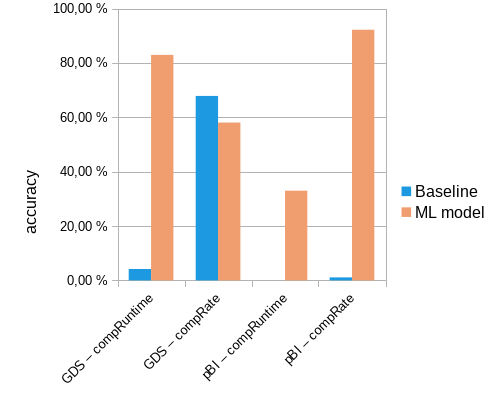
\includegraphics[scale=0.43]{accuracy_param_new_new}
      \caption{Accuracy of algorithm parameter selection (pa).}
    \end{subfigure}
    \\
    \begin{subfigure}{.5\textwidth}
      \centering
      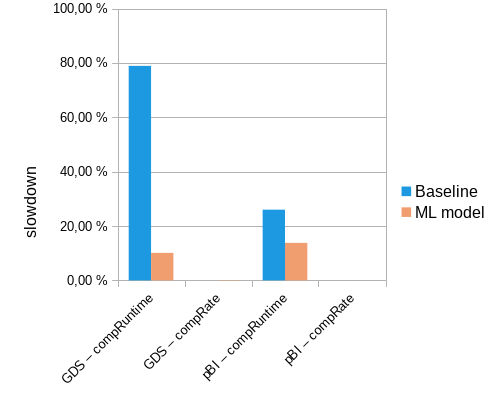
\includegraphics[scale=0.43]{slowdown_param_new_new}
      \caption{Slowdown of incorrect parameter selection (slowdown).}
    \end{subfigure}%
    \caption{Evaluation results against the generated data set (GDS) and Public BI data (pBI) considering the compression rate (compRate) and the compression runtime (compRuntime) as target values.}
    \label{fig:validation-results}
\end{figure}

The validation results presented in figure \ref{fig:validation-results} and its corresponding table \ref{fig:val_tab} show that for the compression runtime as the target value, our ML model performs better than the baseline when using our test data as well as the Public BI data regarding the algorithm selection accuracy, the algorithm parameterization selection accuracy and the slowdown. Considering the compression rate, the baseline performs better for the accuracy of the algorithm parameter selection. The baseline accuracies of 67,85\% for the test data and 1,1\% for the Public BI data are equal to the values of the algorithm selection accuracy. The reason for this lies in the way \emph{StaticBP} works. The combination of an input format of 64 bit and an output format of 8 bit always results in the best compression rate. Thus, if the baseline algorithm, i.e \emph{StaticBP} is chosen and the compression rate is used as target value, the baseline parameterization is always the best. This is also the reason for the corresponding slowdown of 0\%.

\begin{figure}[h]
    \centering
    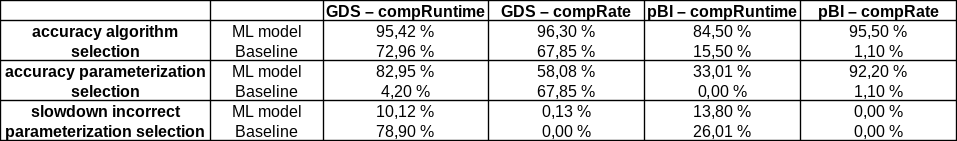
\includegraphics[width = 1\textwidth]{table_results}
    \caption{Validation table.}
    \label{fig:val_tab}
\end{figure}

The GDS is naturally more systematic and contains less outliers than the pBI dataset. Regarding the accuracy of parameterization selection, we note that our ML model performs better on the GDS when trained for the compression runtime. In contrast, it performs better on the pBI dataset when trained for the compression rate.
Due to the fact that the pBI data has different structures and properties, the model has to abstract more from the training data. Predicting the target values is therefore more difficult what results in the lower accuracies for the pBI data set than for the GDS.
Since the compression rate leads to better results for the pBI data in comparison to the compression runtime, we conclude that it is easier for the ML model to predict the compression rate than the compression runtime.
The measurement of the compression runtime is more prone to higher variations in the resulting data. The values for the compression rate on the other hand fluctuate less.

Furthermore, we observed that the ML model always reached better accuracies for the selection of the correct algorithm than for the algorithm's best parameters. The algorithm selection seems to be the easier task for the ML model than the prediction of the parameters. We expected this observation due to the different amount of possible results. While there are at worst 16 possibilities for the algorithm parameters (see Figure \ref{fig:data-sample}), there are only two for the correct algorithm.

Thus far, we evaluated our approach by considering the performance of our ML model as a whole, regardless of certain algorithm parameter combinations. In order to examine which parameter combinations lead to the best prediction results, we calculated the SMAPE for every possible combination of the input format and the output format. We do not consider the maximum bitwidth as it fully depends on the data. There are 16 different algorithm parameter combinations for the GDS. As all integer sequences of the pBI dataset have an input format of 64 bit, therefore only 4 combinations are possible. 
\newpage
\begin{figure}[h]
    \centering
    \begin{subfigure}{.5\textwidth}
      \centering
      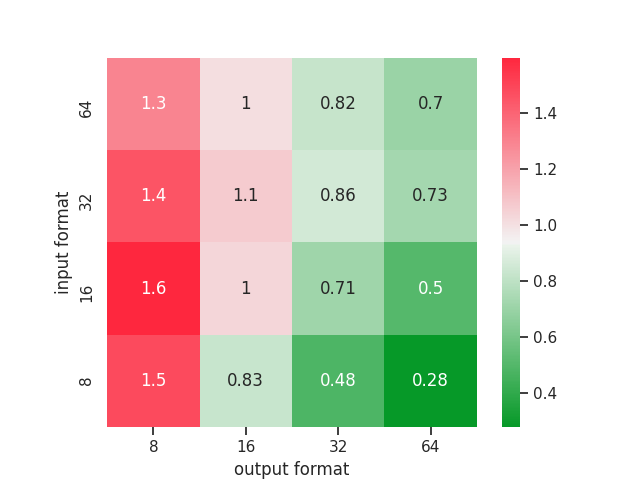
\includegraphics[scale=0.5, trim=4 0 4 4,clip]{heatmap_dynamic_compressionRate_testdata}
      \caption{compression rate}
    \end{subfigure}%
    \begin{subfigure}{.5\textwidth}
      \centering
      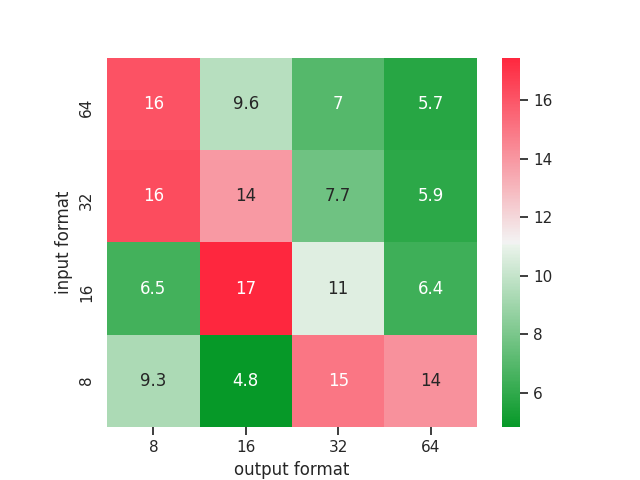
\includegraphics[scale=0.5, trim=4 0 4 4,clip]{heatmap_dynamic_duration_testdata}
      \caption{compression runtime}
    \end{subfigure}%
    \caption{Heatmap (SMAPE in \%) for single parameter combinations on the GDS for \emph{DynamicBP}.}
    \label{fig:heatmaps-single-smapes-tds-dynamic}
\end{figure}
\begin{figure}[h]
    \begin{subfigure}{.5\textwidth}
      \centering
      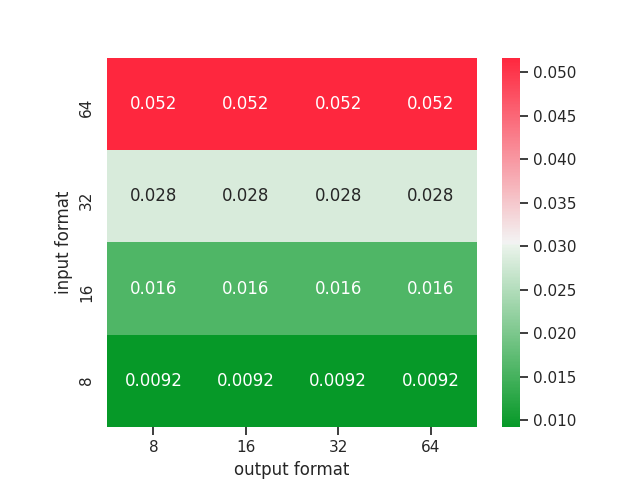
\includegraphics[scale=0.5, trim=4 0 4 4,clip]{heatmap_static_compressionRate_testdata}
      \caption{compression rate}
    \end{subfigure}%
    \begin{subfigure}{.5\textwidth}
      \centering
      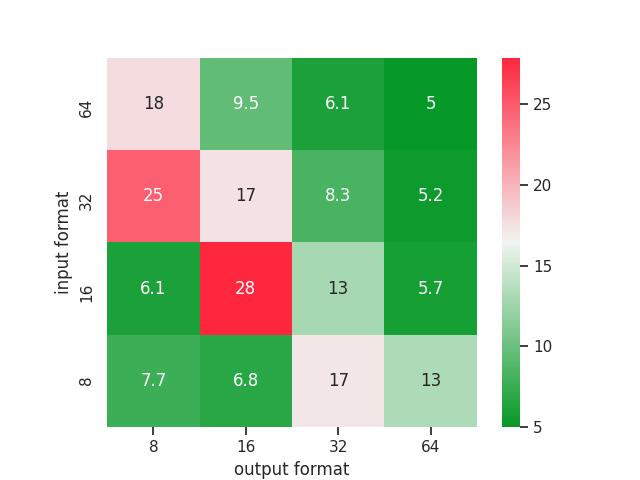
\includegraphics[scale=0.5,trim=4 0 4 4,clip]{heatmap_static_duration_testdata}
      \caption{compression runtime}
    \end{subfigure}%
    \caption{Heatmap (SMAPE in \%) for single parameter combinations on the GDS for \emph{StaticBP}.}
    \label{fig:heatmaps-single-smapes-tds-static}
\end{figure}

Figures \ref{fig:heatmaps-single-smapes-tds-dynamic} and \ref{fig:heatmaps-single-smapes-tds-static} show the SMAPE values for each possible parameter combination within the GDS. Regarding the compression runtime, the lowest SMAPE values representing better prediction results have been calculated for combinations of small input and output formats on the one hand, and for combinations of large input and output formats on the other hand. The highest SMAPE values indicating worse prediction results were determined for combinations of small input formats with large output formats and vice versa.
This behavior applies equally for both algorithms. The prediction quality of the ML model hence increases if either combinations of large input and output parameters or combinations of small input and output parameters are considered.
If a new data set is passed to the ML model in order to predict the best fitting algorithm and its parameters with the compression runtime as target value, it is useful to adjust the possible range of output format values depending on the input format(s) of the data being analysed.\\ 
In contrast to that, the prediction results of the ML model using the compression rate as target values show a different behavior for both algorithms. While the ML model performs better for \emph{DynamicBP} the larger the value for the output format, the output format has no influence on the prediction result of the ML model for \emph{StaticBP}. The reason is that the compression rate of \emph{StaticBP} is determined statically with the input format and the max bitwidth of the integer sequence.

\begin{figure}[h]
    \centering
    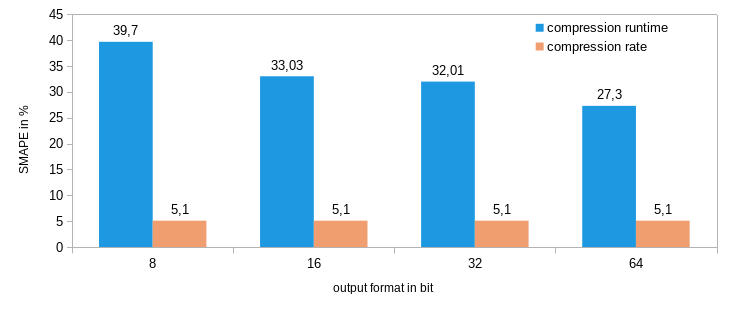
\includegraphics[width=\textwidth]{bar_chart_pbi_smapes_staticBP}
    \caption{SMAPE barchart for possible output formats (pBI dataset, \emph{StaticBP}, input format = 64 bit).}
    \label{fig:smapes_pbi_static}
\end{figure}
\begin{figure}[h]
    \centering
    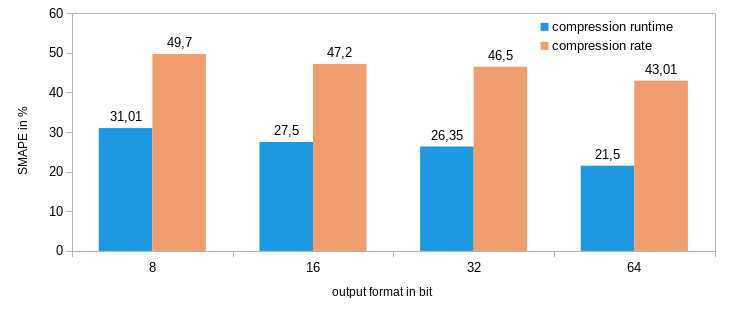
\includegraphics[width=\textwidth]{bar_chart_pbi_smapes_dynamicBP}
    \caption{SMAPE barchart for possible output formats (pBI dataset, \emph{DynamicBP}, input format = 64 bit).}
    \label{fig_smapes_pbi_dynamic}
\end{figure}

Figure \ref{fig:smapes_pbi_static} and \ref{fig_smapes_pbi_dynamic} show heatmaps containing the SMAPE values of each possible parameter combinations within the pBI data set. We can observe a similar behavior to the GDS. For every target value and algorithm, the SMAPE decreases the higher the output format is. The input format of the pBI dataset is 64 for every integer sequence. The increase in prediction quality with larger output format values fits the observation made for the GDS for an input format of 64 bit regardless the target value.   

One exception is the compression rate when using \emph{StaticBP}. Figure \ref{fig:smapes_pbi_static} shows again an equal SMAPE value for every possible output format. The reason is the same as already found for the GDS, as the functionality of the algorithms is the same for all data. 
\newpage
\section{Feature Importance}
Being able to interpret the ML models of our \emph{Learned Selection Strategy for Lightweight Integer Compression Algorithm Parameterizations} requires the consideration of feature importance. The importance of a certain feature indicates what influence it has on the model's quality. There are different ways to determine the importance of a feature. The indicator we used is the permutation feature importance \cite{Breiman2013}. 

To determine the individual importance, the following process is applied successively to every feature \cite{Breiman2013}. Firstly, the feature values get shuffled randomly over all samples which results in a decrease of the quality of the ML model. As the shuffling process breaks the relationship between the feature and the target value, the decrease is an indicator how much the target value depends on the feature. This process leads to a value indicating the decrease of the model quality and hence the importance of the feature (feature importance value).\\
We used the implementation of scikit-learn\footnote{https://scikit-learn.org/stable/modules/permutation\_importance.html, last access: 01.10.2021} which is outlined as follows:
Given the ML model \emph{m} and the training data set \emph{D}, a reference score \emph{s} is calculated indicating the quality of the model. Now, the values for each feature \emph{j} get shuffled multiple times \emph{k} which results in a corrupted version of the data set $\widetilde{D}_{j,k}$.
Now, the reference score $s_{j,k}$ is calculated for the model \emph{m} on the corrupted data set $\widetilde{D}_{j,k}$.
The importance of each feature is the difference of the reference score belonging to the original data set and the average of the corrupted reference scores.
\begin{equation}
    i_{j} = s - \frac{1}{K}\sum_{k=1}^{K} s_{k,j}
\end{equation}
\begin{figure}[h]
   \centering
   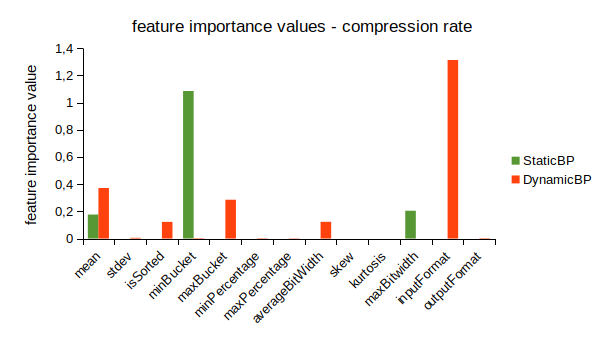
\includegraphics[scale=0.8]{feature_importance_rate}
   \caption{Feature importances for compression rate as target value.}
   \label{fig:feature_importances_compression_rate}
\end{figure}

Figure \ref{fig:feature_importances_compression_rate} shows that the ML model for \emph{StaticBP} mostly depends on the minBucket feature and the maxBitwidth feature when trained to predict the compression rate. The model for \emph{DynamicBP} mostly depends on the input format. Both observations are indicators that the ML models represent the behavior of the algorithms.
Considering \emph{StaticBP}, the block size is fixed and determined by the maxBitwidth parameter. As the minBucket feature is inversely proportional to the maxBitwidth feature, the model can derive the algorithm behavior from both features.
Regarding \emph{DynamicBP}, the bit width of a block's largest value is chosen to represent all data elements in the block \cite{Woltmann2021}. The input format correlates with the bit width of a block's largest value which is the reason for its importance.
\begin{figure}[h]
    \centering
    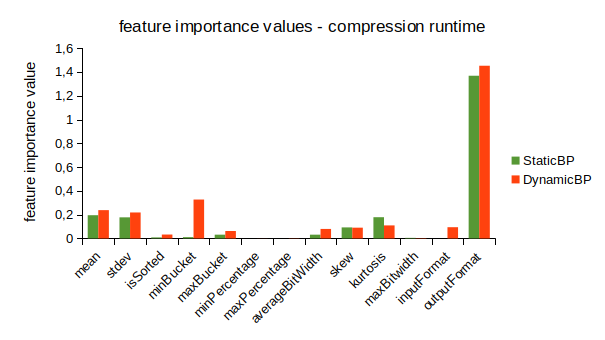
\includegraphics[scale=0.8]{feature_importance_runtime}
    \caption{Feature importances for compression runtime as target value.}
    \label{fig:feature_importances_compression_runtime}
\end{figure}

Figure \ref{fig:feature_importances_compression_runtime} shows the feature importances on the ML models when trained on the compression runtime. For both \emph{DynamicBP} and \emph{StaticBP} the outputFormat is the feature with the highest feature importance value. The output format is an indicator for the length of the integer sequence being compressed. Hence we can conclude that the longer the sequences are, the more time it takes to compress them which is an intuitive behavior. This is also the reason why it was necessary to scale the predicted compression runtime value of the pBI dataset accordingly.
Besides the output format, the features mean, stdev and minBucket have relatively high feature importance values. All three features are correlated to the size of the integer values the sequence contains. In addition to the length of the sequence, the size of the values also affects the compression runtime.

\section{Conclusion}
The evaluation of the \emph{Learned Selection Strategy for Lightweight Integer Compression Algorithm Parameterizations} has shown that its usage results in better compression results (i.e compression runtime and compression rate) than the application of the simplest approach for generated data as well as for real world data. Additionally, our learned approach results in a lower slowdown if the incorrect parameterization is chosen than the most simple approach does.